\newcolumntype{L}[1]{>{\raggedright\arraybackslash}p{#1}}


\section{Testing}
To ensure the reliability and correctness of the Odyssey Travel Agency Software, a structured testing methodology was followed throughout the development lifecycle. This methodology included four primary types of testing:

\begin{itemize}
    \item \textbf{Unit Testing:} Conducted on individual functions and components such as the login system, package listing, and hotel selection module. JavaScript-based unit tests were created using testing libraries like Jest.
    
    \item \textbf{Integration Testing:} Focused on verifying the interaction between modules. For example, integration of the package selection page with the booking module and the payment gateway was carefully validated.
    
    \item \textbf{System Testing:} The complete software was tested in a controlled environment to ensure it meets functional and non-functional requirements. This was done using the deployed system with sample user flows.
    
    \item \textbf{User Acceptance Testing (UAT):} Selected users were invited to test the application from a real-world user perspective. Feedback was collected and evaluated to improve usability, performance, and correctness.
\end{itemize}

\section{Unit Testing}
Unit testing was conducted to test individual modules in isolation. The main goals were to verify correctness of logic, detect early bugs, and ensure maintainability.

\begin{itemize}
    \item Each React component and backend API endpoint was tested using automated test cases.
    \item Modules like authentication, registration, tour guide assignment, and package search were tested individually.
    \item Edge cases were tested such as invalid email formats, empty form submissions, and duplicate user entries.
\end{itemize}

Sample assertion example for user registration:
\begin{verbatim}
expect(registerUser("test@mail.com", "password123")).toBeTruthy();
\end{verbatim}

\section{Integration Testing}
Integration testing was carried out to ensure seamless communication between various components.

\begin{itemize}
    \item Verified data flow from front-end forms to the backend database via the Express API.
    \item Ensured synchronization between hotel/flight selection and the final booking confirmation.
    \item Checked for error handling during API failures or slow network conditions.
\end{itemize}

For example, a package booked by the user was tested to ensure the details were stored correctly and retrievable under the user's booking history.

\section{System Testing}
System testing evaluated the behavior of the complete application. Both functional and non-functional requirements were validated.

\begin{itemize}
    \item Complete booking workflows were tested – from login to payment confirmation.
    \item Admin panel functionalities such as package CRUD operations and tour guide assignment were fully validated.
    \item Tested across multiple browsers (Chrome, Firefox, Edge) to ensure UI consistency.
\end{itemize}

All modules worked correctly when deployed via a local server using XAMPP and MySQL database integration.

\section{User Acceptance Testing}
UAT was performed with a group of 5 users including students and travelers. Their task was to use the system and provide usability feedback.

\begin{itemize}
    \item Majority found the interface intuitive and easy to navigate.
    \item Suggestions were made to improve hotel filtering and add date-based filtering in future versions.
    \item No major bugs were reported during this phase, indicating system readiness.
\end{itemize}

User feedback was recorded and considered for future iteration plans.

\section{Test Cases and Results}
A set of planned test cases were executed to validate the system’s critical functions. A sample of these test cases is summarized below:


\begin{longtable}{|L{6cm}|L{10cm}|}
    \caption{Project Information Table} \label{tab:project_info} \\
    \hline
    \textbf{Project Name} & Odyssey Travel Agency Software
    \\ \hline
    \textbf{Module Name} & Software Testing \\ \hline
    \textbf{Created By} & Hafizur Rahman Sakib and Arnab Shikder \\ \hline
    \textbf{Date of Creation} & 17.02.2024 \\ \hline
    \textbf{Date of Review} & 02.05.2025 \\ \hline
  \end{longtable}

\begin{longtable}[
    ]{
      |L{1.3cm}|L{2.2cm}|L{2.0cm}|L{2.5cm}|L{2.0cm}|L{2.2cm}|L{1.3cm}|
    }
    \caption{Comprehensive Test Case Execution Table for Odyssey Travel Agency Software} \label{tab:test_cases} \\
    \hline
    \textbf{Test Case ID} & 
    \textbf{Test Scenario} & 
    \textbf{Pre-Condition} & 
    \textbf{Test Steps} & 
    \textbf{Test Data} & 
    \textbf{Expected Result} & 
    \textbf{Status} \\
    \hline
    \endfirsthead
    \caption[]{Comprehensive Test Case Execution Table (Continued)} \\
    \hline
    \textbf{Test Case ID} & 
    \textbf{Test Scenario} & 
    \textbf{Pre-Condition} & 
    \textbf{Test Steps} & 
    \textbf{Test Data} & 
    \textbf{Expected Result} & 
    \textbf{Status} \\
    \hline
    \endhead
    \hline
    \endfoot
    \footnotesize % Use smaller font size for better fit
    TC001 & User Login & User is registered & Enter email and password, click login & Email: user@mail.com, Password: 1234 & Dashboard is shown & Pass \\ \hline
    TC002 & Add New Package & Admin is logged in & Go to ``Add Package'', fill form, click submit & Package Name: Beach Trip & Package added successfully & Pass \\ \hline
    TC003 & Invalid Booking & User logged in & Try booking a package skipping hotel selection & N/A & Error message displayed & Pass \\ \hline
    TC004 & Payment Processing & User is on payment page & Enter valid card details and submit & Card No: 4111 1111 1111 1111 & Payment confirmation message & Pass \\ \hline
    TC005 & Session Timeout & User is logged in & Wait 30 minutes without interaction & Timer: 30 mins & Session timeout message shown & Pass \\ \hline
    TC006 & Search Function & User is on homepage & Type keyword in search bar and click search & Keyword: Cox's Bazar & Related packages shown & Pass \\ \hline
    TC007 & Unauthorized Access & User is logged out & Try accessing \texttt{/admin} directly in browser & URL: /admin & Access denied or redirected to login & Pass \\ \hline
    TC008 & User Registration & N/A & Fill in name, email, password, and submit & Name: John Doe, Email: john@mail.com, Password: 1234 & Registration successful message & Pass \\ \hline
    TC009 & Password Reset & User is on login page & Click ``Forgot Password'', enter email, click submit & Email: john@mail.com & Password reset link sent to email & Pass \\ \hline
    TC010 & Edit Package & Admin is logged in & Go to ``Edit Package'', change details, click save & Package ID: 101, New Price: 5000 & Package details updated successfully & Pass \\ \hline
    TC011 & Verify User Logout & User is logged in & Click logout button & N/A & User is logged out & Pass \\ \hline
    TC012 & Invalid Payment & User is on payment page & Enter invalid card details and submit & Card No: 1234 5678 9012 3456 & Error message displayed & Pass \\ \hline
    TC013 & Change User Role & Admin is logged in & Go to user list, select user, change role, click save & User ID: 102, New Role: Admin & User role updated successfully & Pass \\ \hline
    TC014 & User Profile Update & User is logged in & Go to profile page, update name, click save & Name: John Doe $\to$ Jane Doe & Profile updated successfully & Pass \\ \hline
    TC015 & Package Filter & User is on homepage & Apply filters by location and price & Location: Cox's Bazar, Price Range: 3000--5000 & Filtered packages are shown & Pass \\ \hline
    TC016 & Cancel Booking & User is logged in, has a confirmed booking & Go to bookings, select booking, click cancel & N/A & Booking canceled successfully & Pass \\ \hline
    TC017 & Admin Login Attempt & Admin is registered & Enter invalid email or password & Email: admin@mail.com, Password: wrongpassword & Error message displayed & Pass \\ \hline
    TC018 & Package Booking Limit & User is logged in & Try booking a package with exceeded limit & Package Name: Deluxe Tour, Max Bookings: 10 & Error message displayed & Pass \\ \hline
  \end{longtable}
\section{Bug Tracking and Resolution}
Throughout development, bugs were tracked using GitHub Issues. Each bug was logged with the following attributes: ID, title, severity (High/Medium/Low), module affected, and resolution status.

\begin{itemize}
    \item Critical bugs like broken redirects and duplicate booking entries were prioritized.
    \item Weekly triage meetings were held to resolve open bugs collaboratively.
    \item Bugs were documented and tested again after fixes were applied.
\end{itemize}

An example bug entry:
\begin{itemize}
    \item \textbf{ID:} \#24
    \item \textbf{Title:} Booking confirmation not loading
    \item \textbf{Severity:} High
    \item \textbf{Status:} Fixed in Sprint 3
\end{itemize}

\section{Performance and Load Testing}
Performance testing focused on response time, page load time, and system behavior under simulated concurrent users.

\begin{itemize}
    \item Simulated 20 concurrent users performing bookings simultaneously.
    \item Response time remained under 2 seconds for 95\% of operations.
    \item Load testing confirmed the Node.js backend and MySQL database handled concurrent transactions reliably.
\end{itemize}

Future improvements may include caching and CDN integration to boost performance further.

\section{Security Testing}
To ensure data integrity and user protection, security testing was conducted.

\begin{itemize}
    \item Passwords stored in encrypted format using bcrypt.
    \item User inputs validated server-side to prevent SQL Injection and XSS attacks.
    \item JWT-based authentication ensured secure access to protected endpoints.
    \item HTTPS enforced during deployment simulation to protect data in transit.
\end{itemize}

These steps ensured compliance with basic web security standards.

The testing phase validated that the Odyssey Travel Agency Software met all functional and non-functional requirements. It performed reliably across different scenarios, resisted invalid input, and provided a secure and user-friendly interface. The successful completion of unit, integration, system, and acceptance testing confirmed the system's readiness for deployment and future scaling.

\section{Result}

This section demonstrates key frontend pages of the application, covering both user and admin perspectives.

\subsection*{User Interface Screens}

\begin{figure}[H]
    \centering
    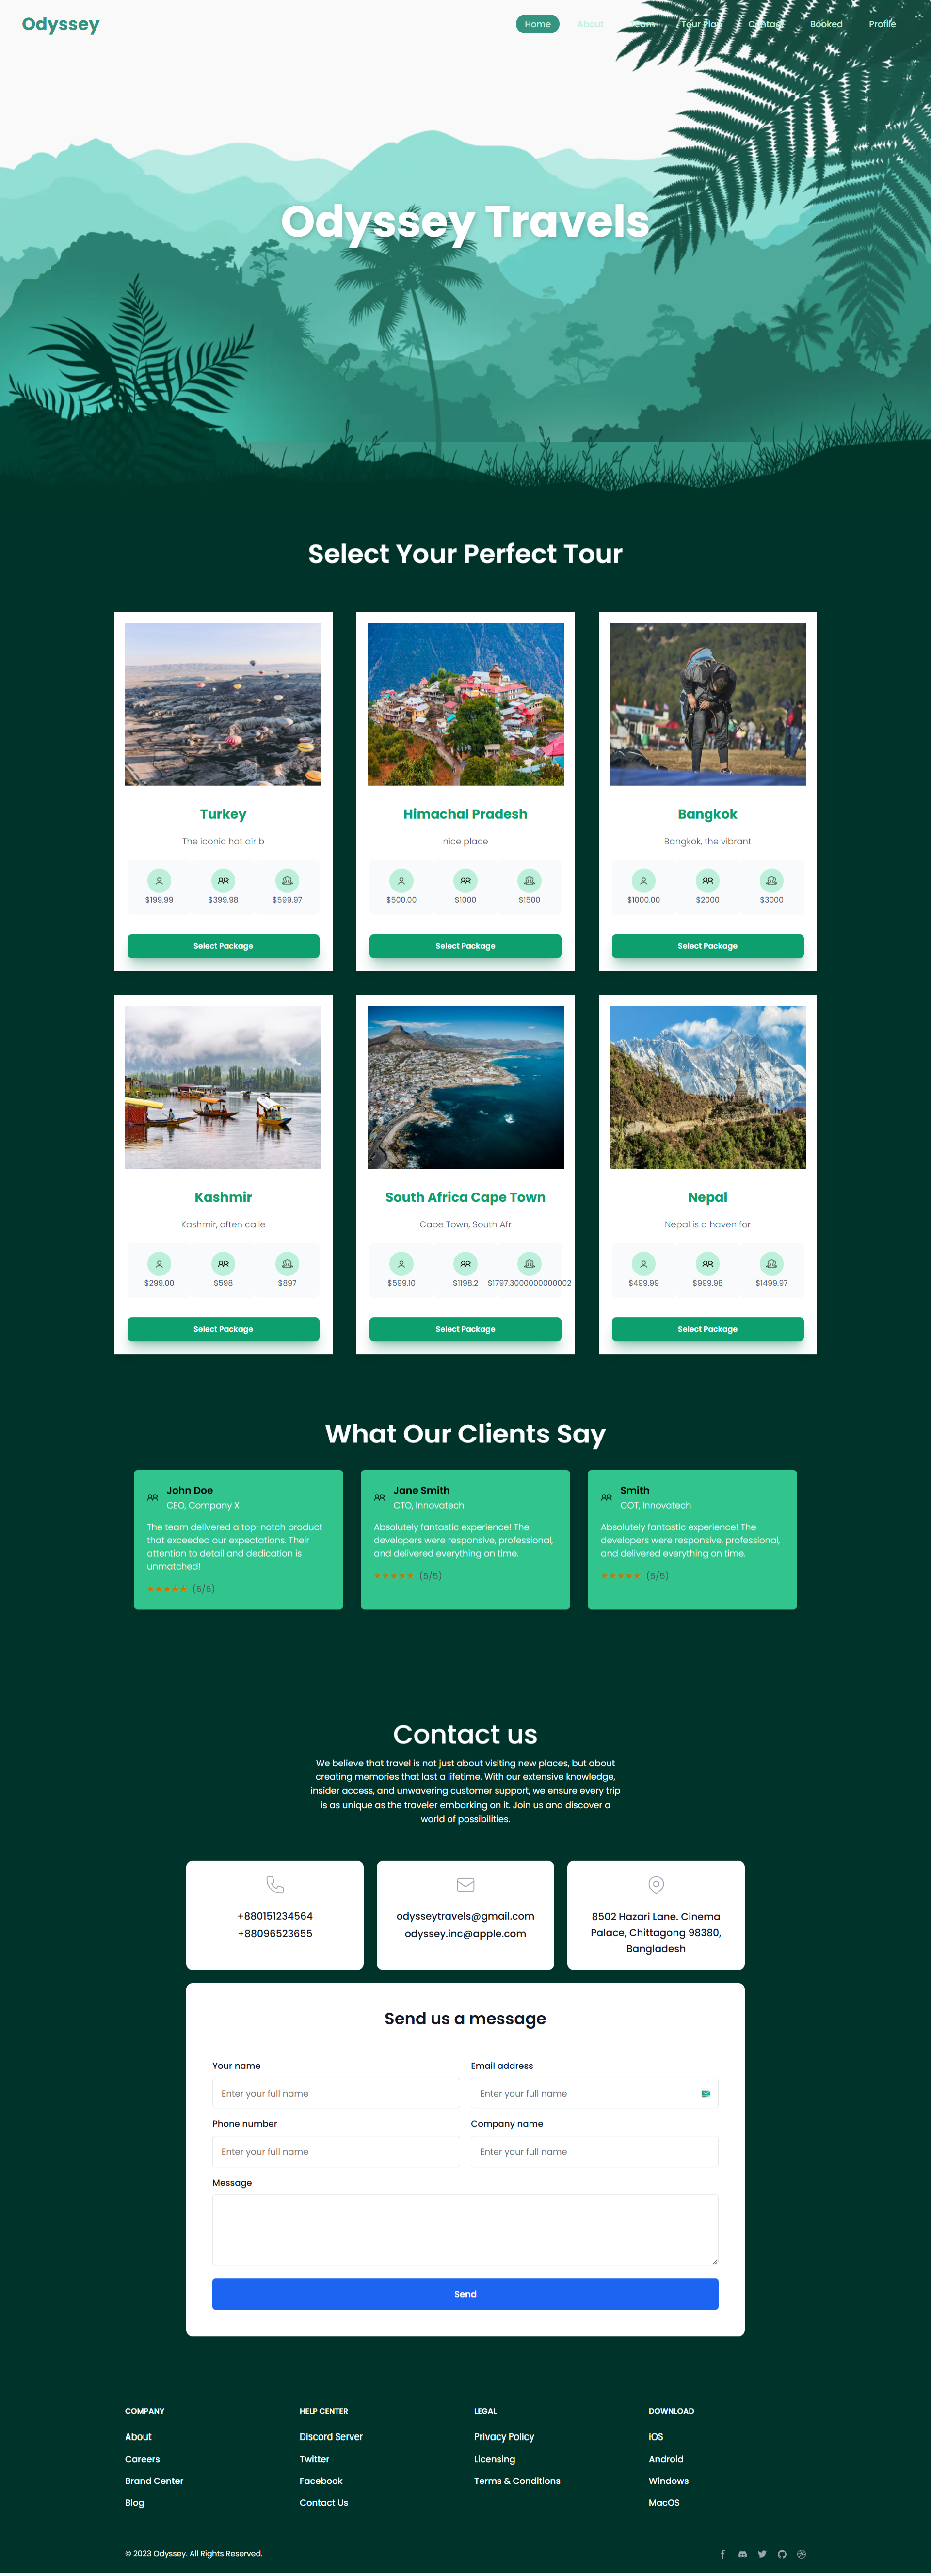
\includegraphics[width=0.95\textwidth]{./figures/frontend/1.png}
    \caption{Homepage}
    \label{fig:homepage}
\end{figure}

\begin{figure}[H]
    \centering
    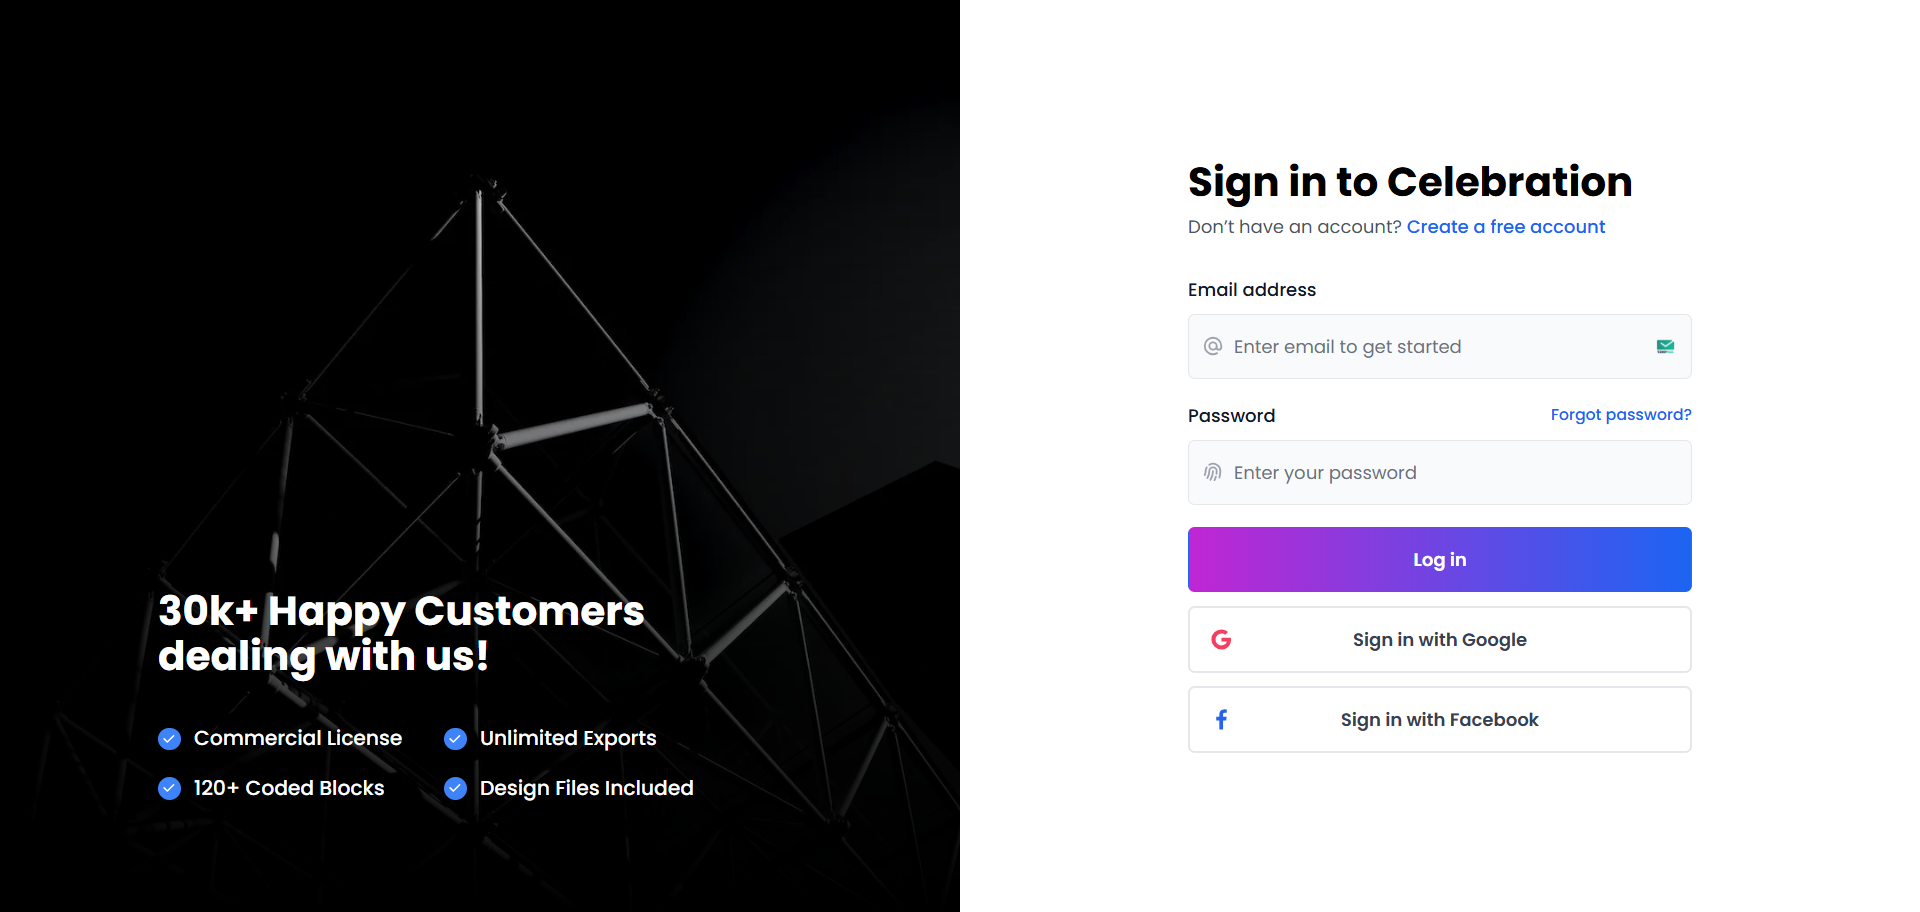
\includegraphics[width=1.0\textwidth]{./figures/frontend/2.png}
    \caption{Login Page}
    \label{fig:login_page}
\end{figure}

\begin{figure}[H]
    \centering
    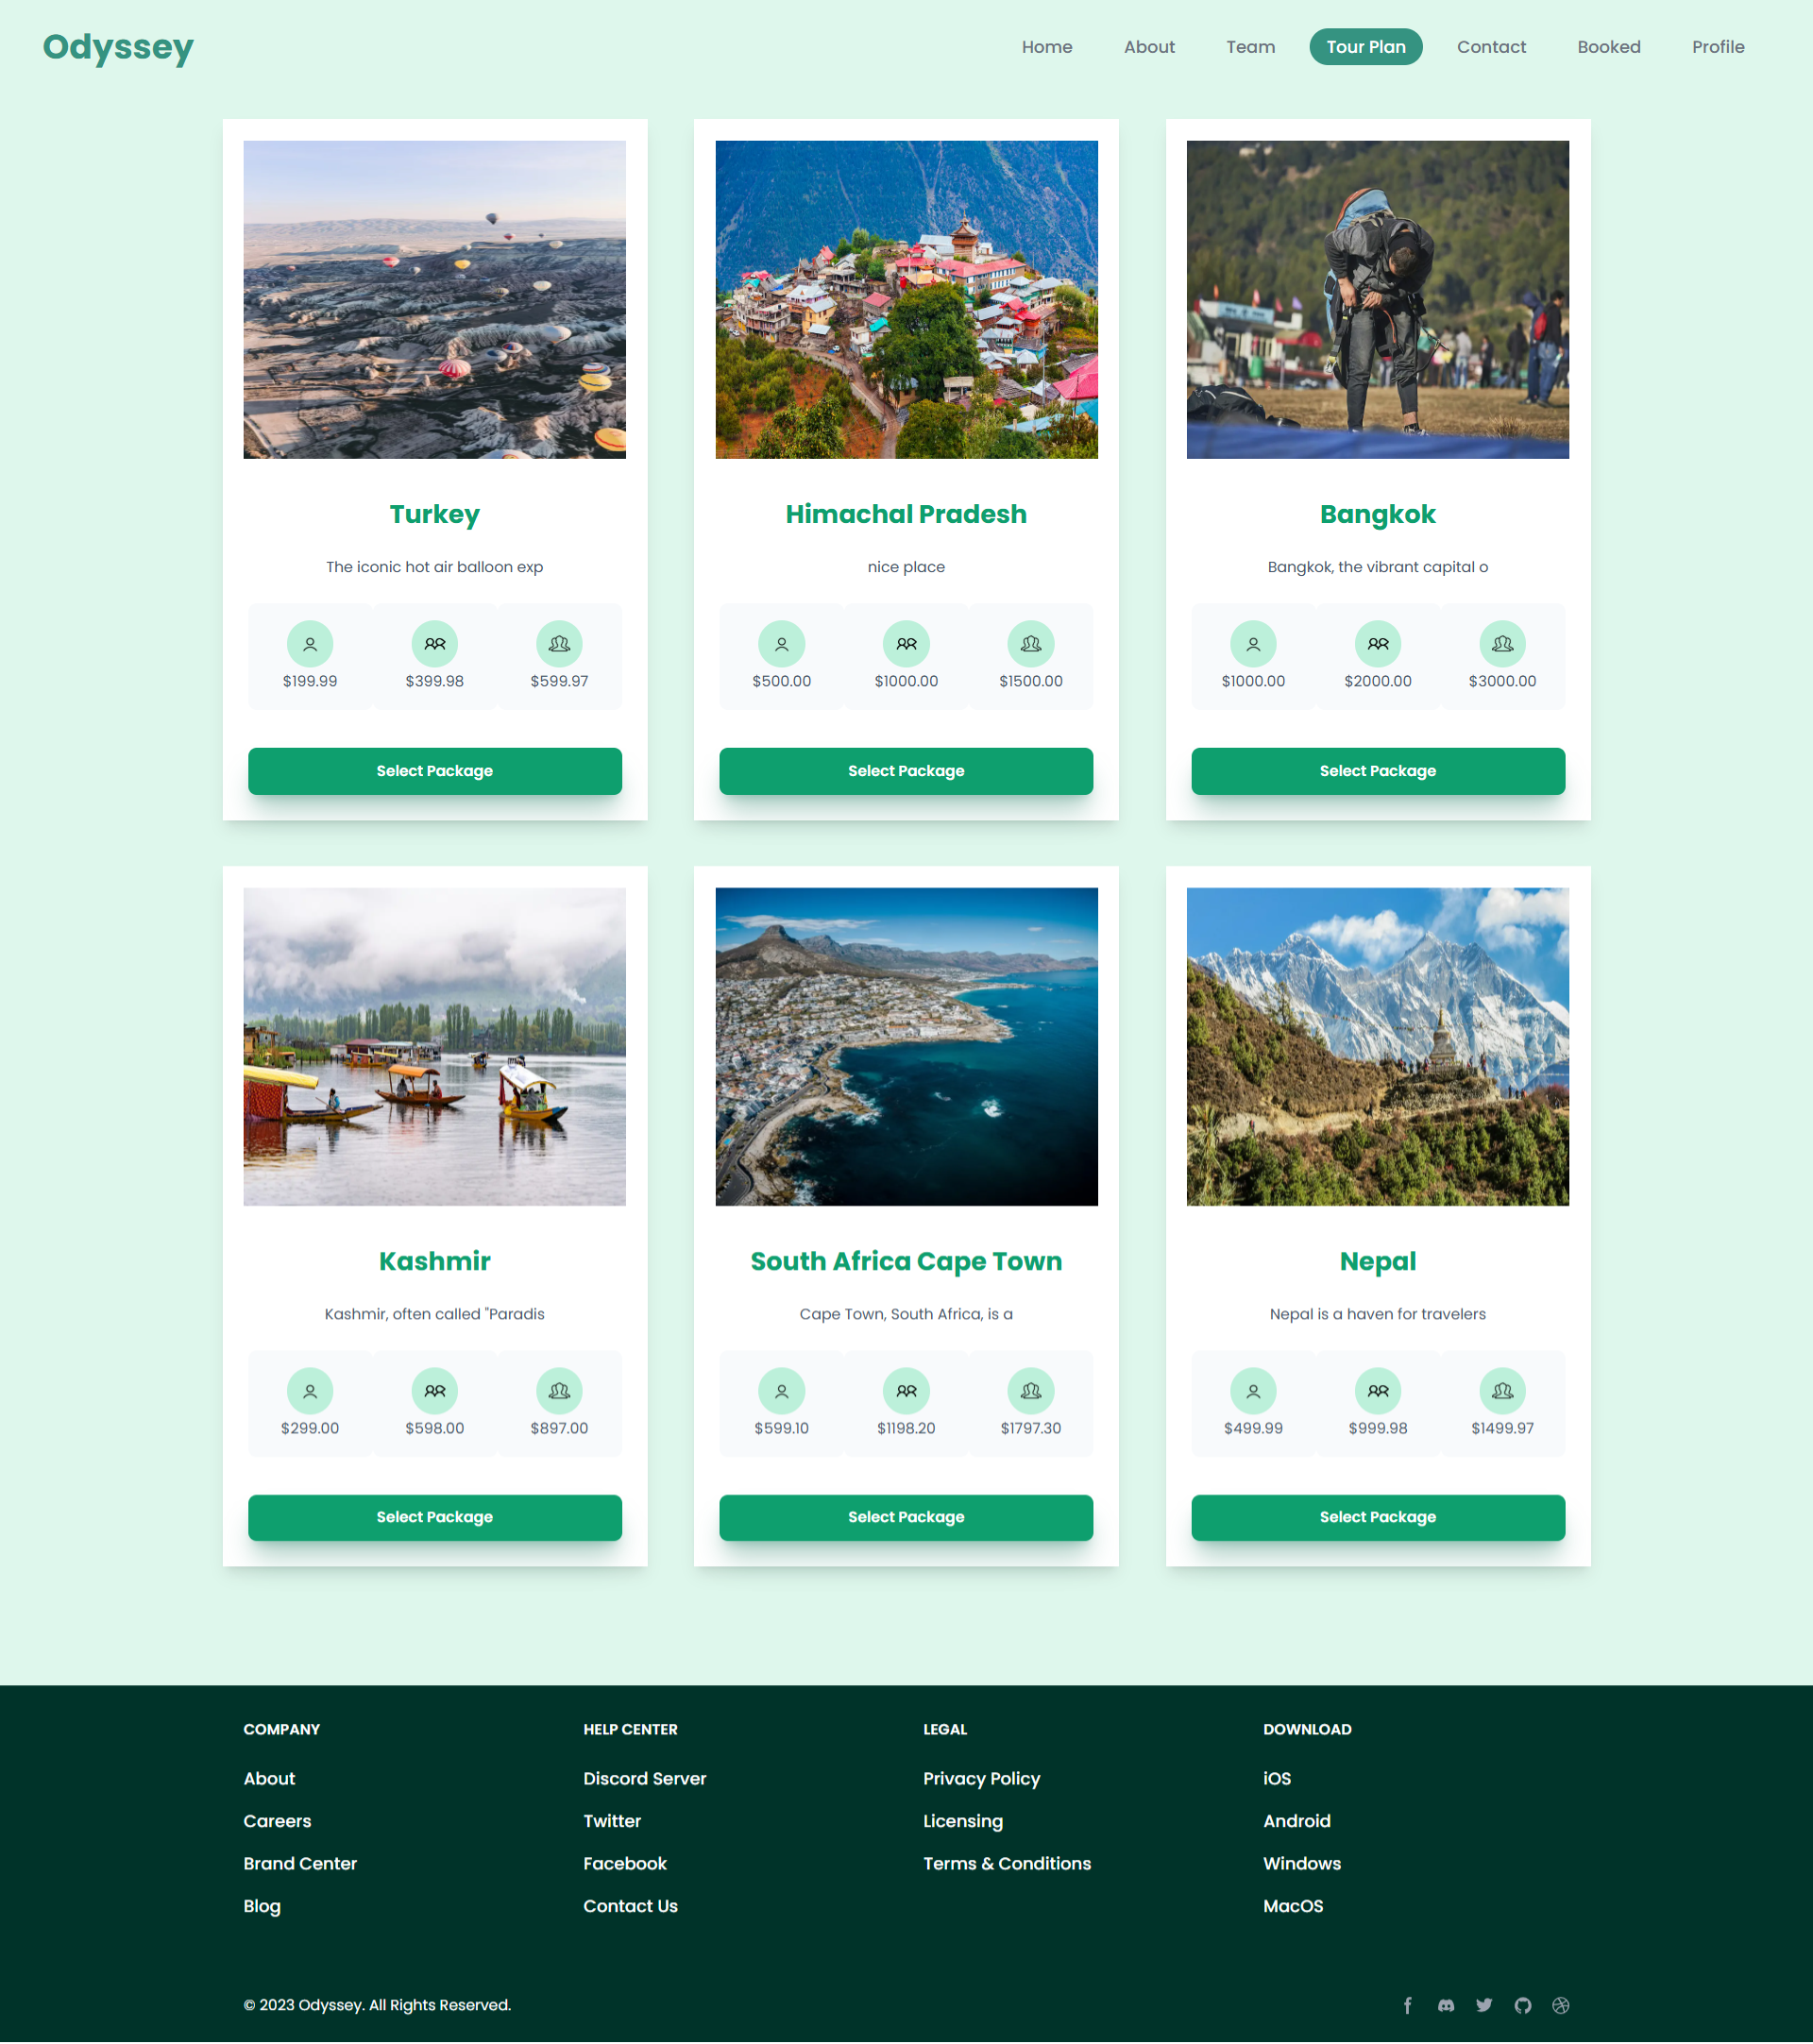
\includegraphics[width=0.95\textwidth]{./figures/frontend/3.png}
    \caption{Tour Plan Page}
    \label{fig:tour_plan}
\end{figure}

\begin{figure}[H]
    \centering
    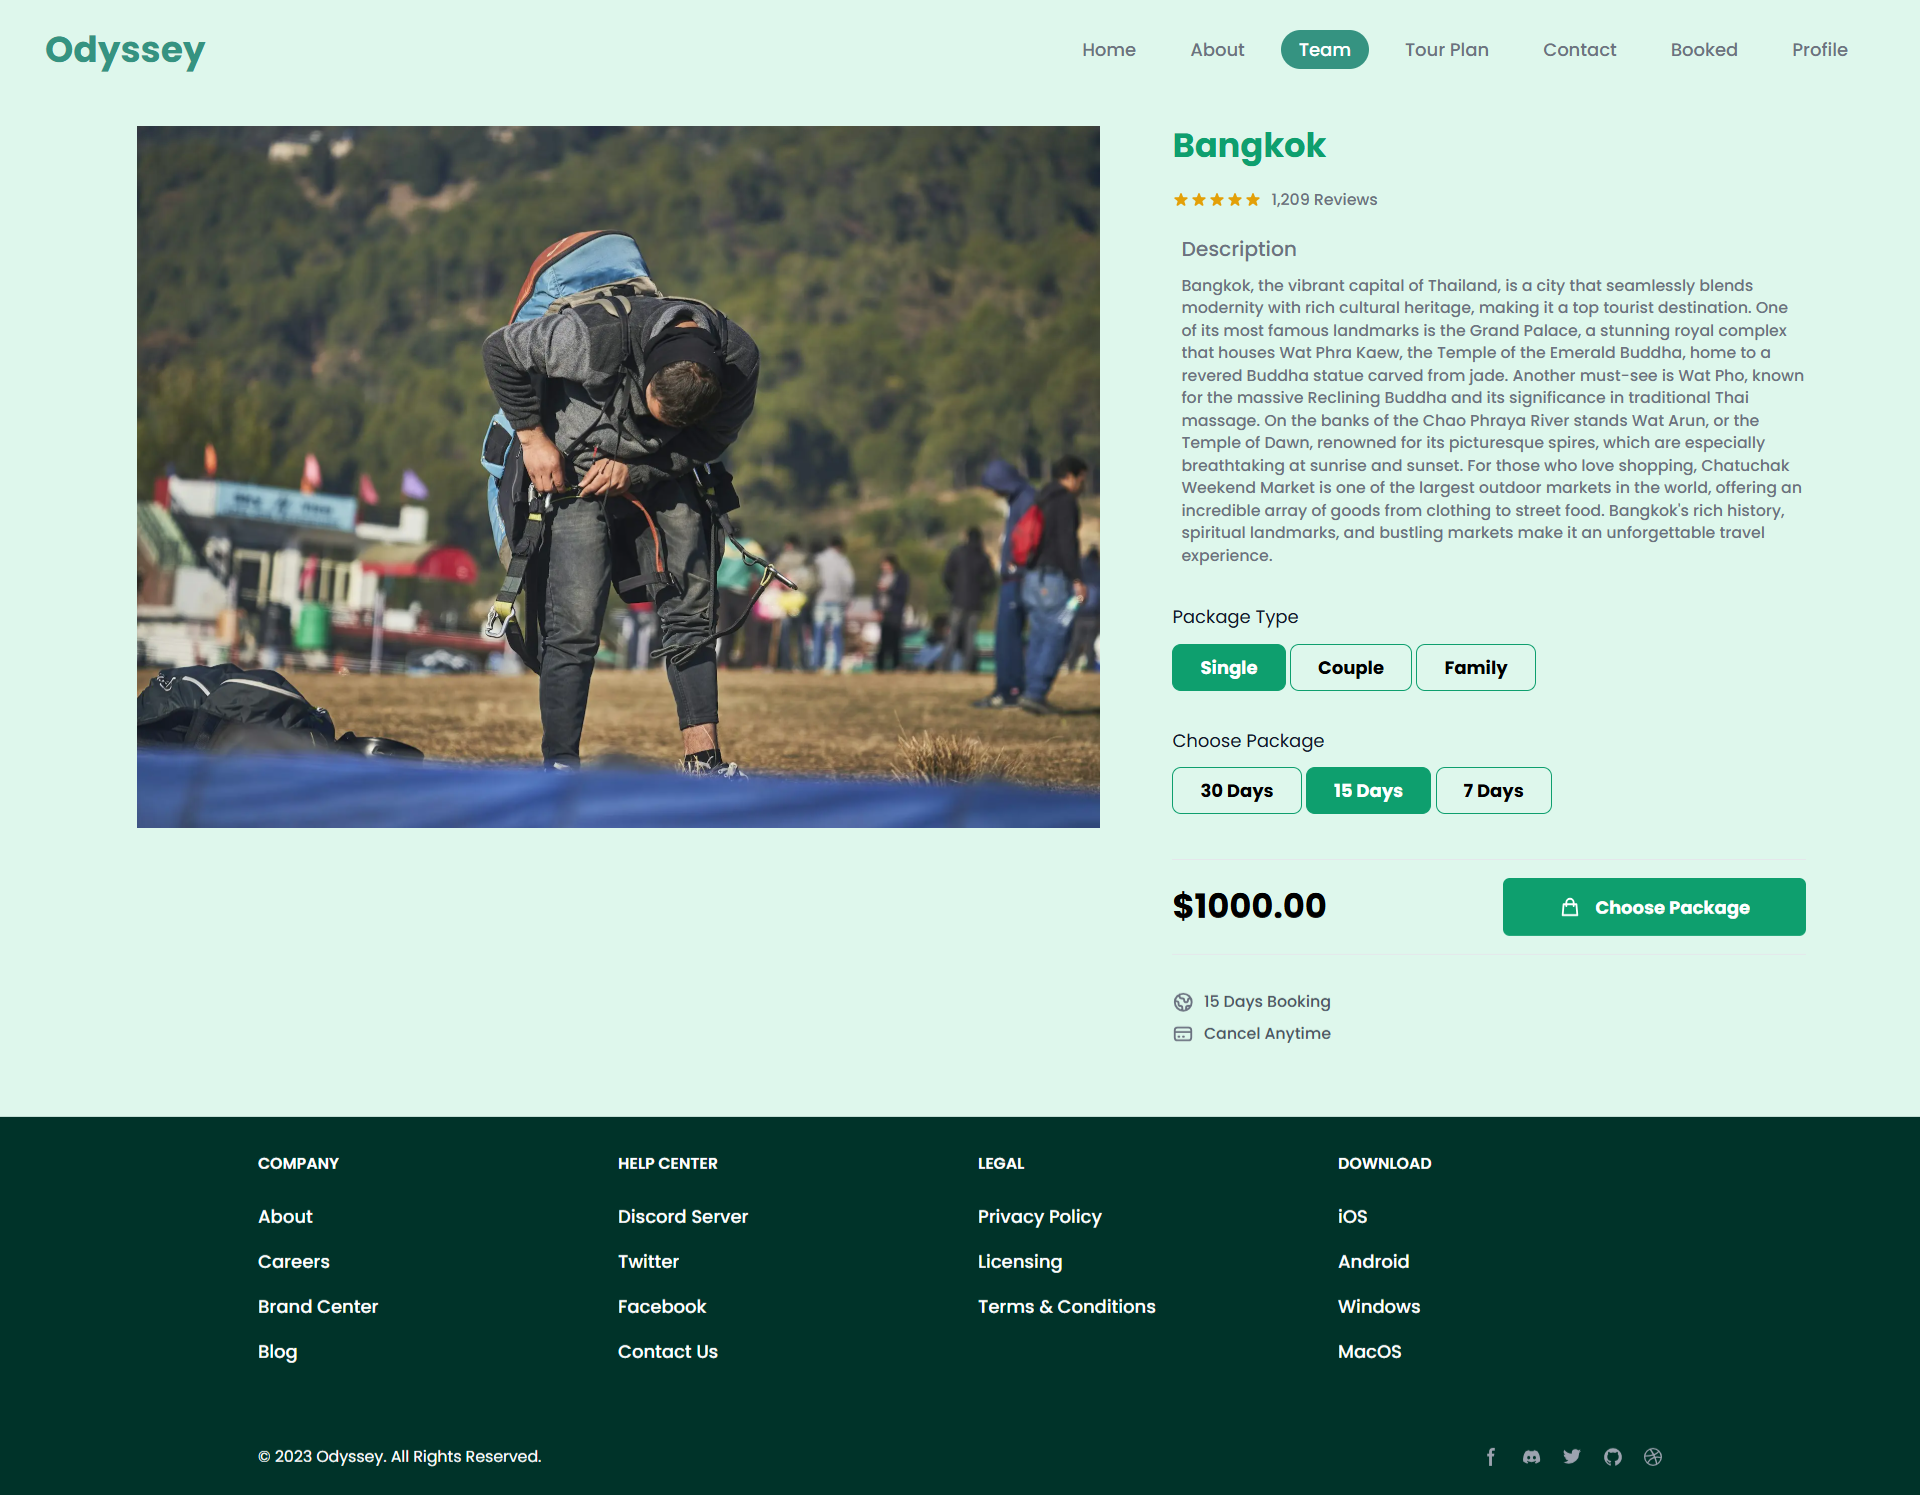
\includegraphics[width=0.95\textwidth]{./figures/frontend/4.png}
    \caption{Package Details Page}
    \label{fig:package_details}
\end{figure}

\begin{figure}[H]
    \centering
    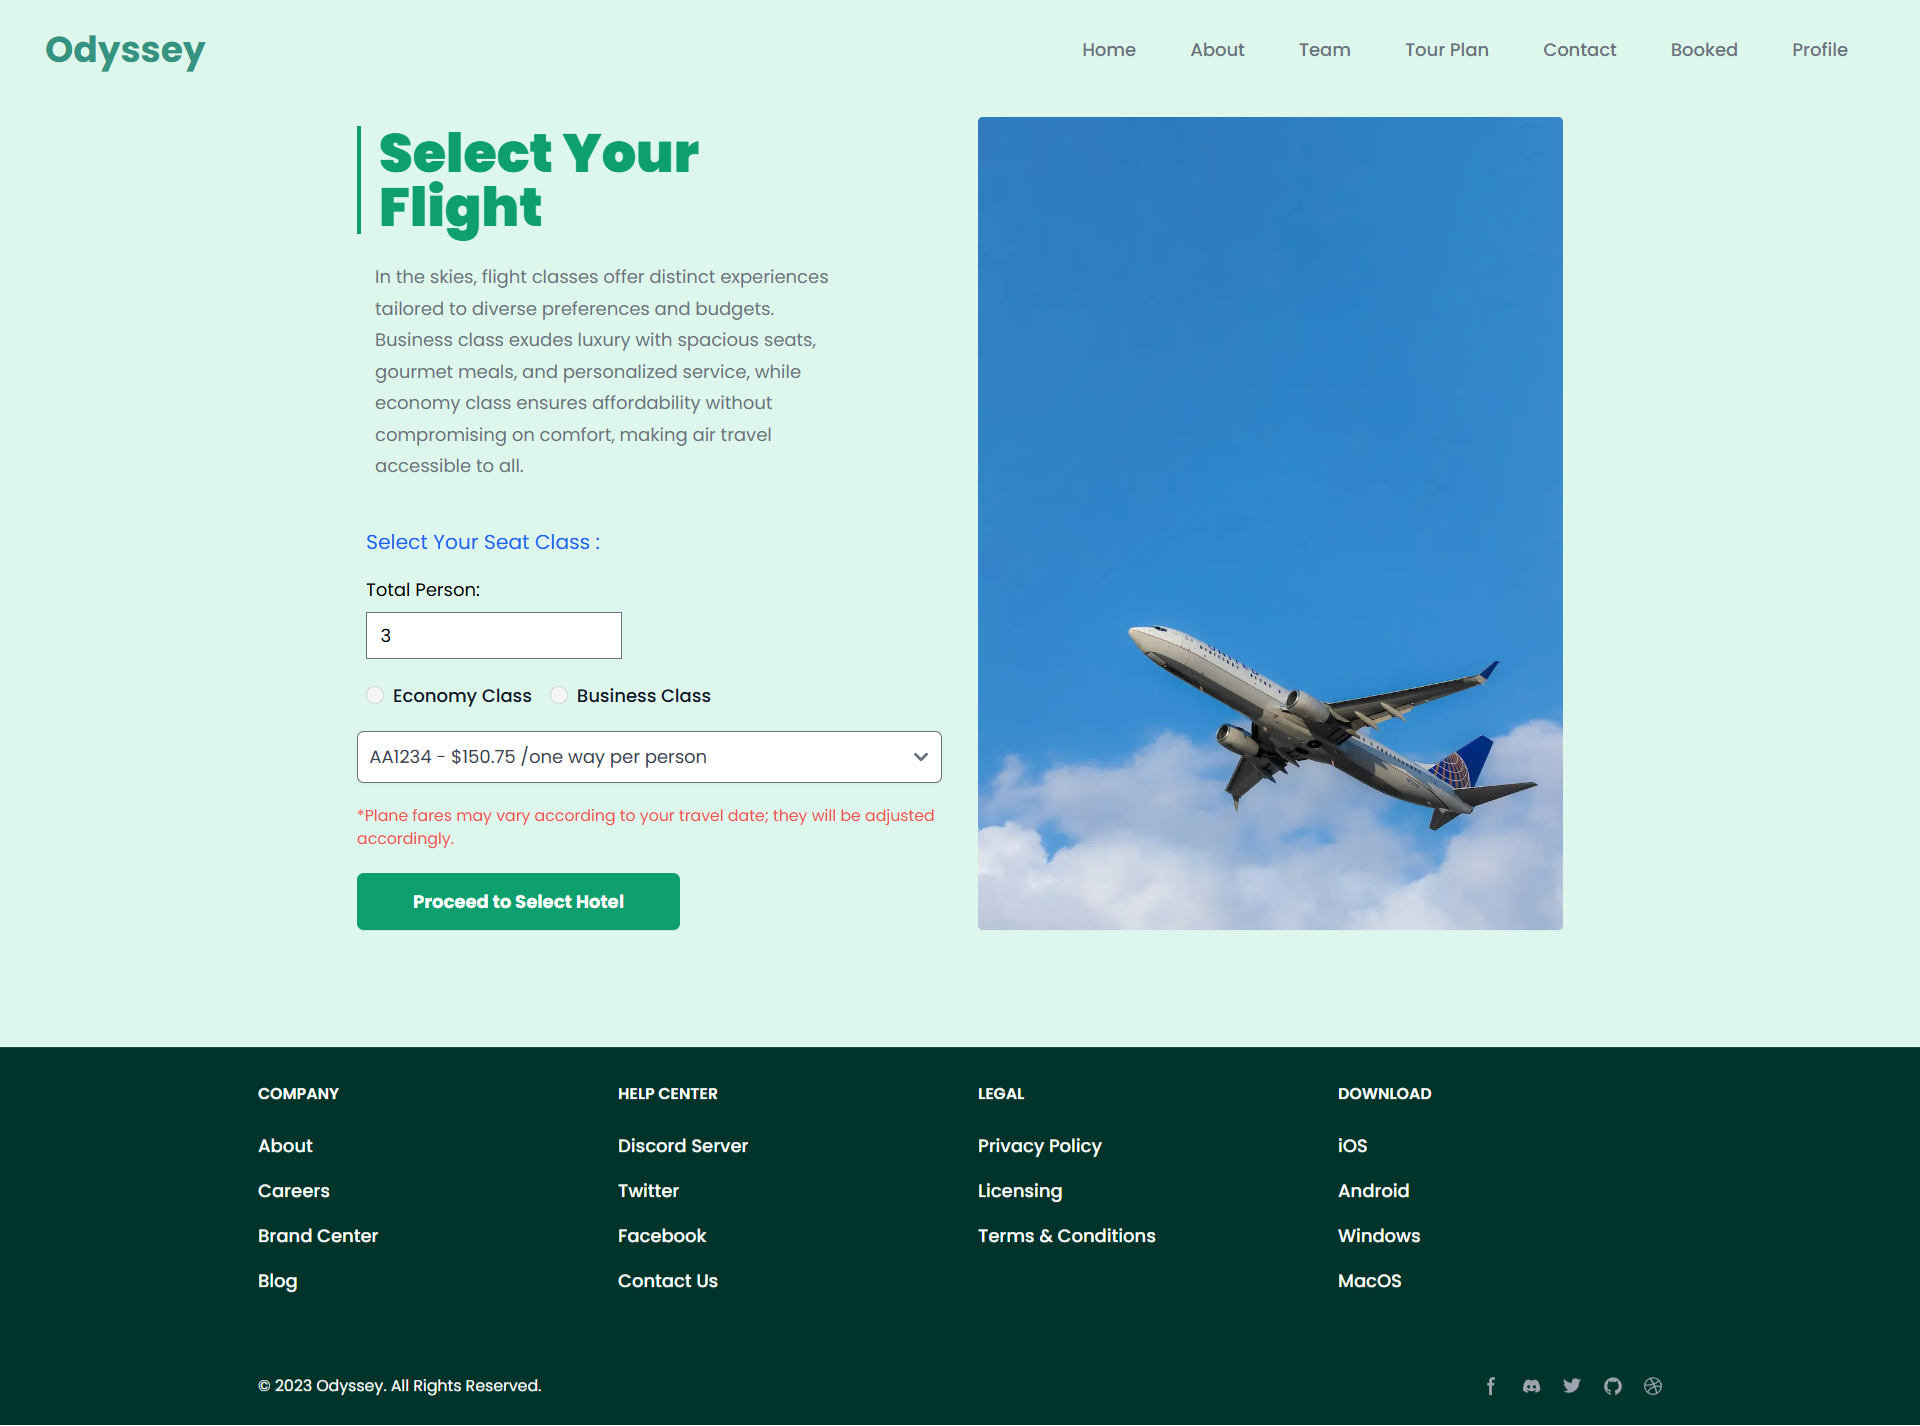
\includegraphics[width=0.95\textwidth]{./figures/frontend/5.png}
    \caption{Select Flight Page}
    \label{fig:select_flight}
\end{figure}

\begin{figure}[H]
    \centering
    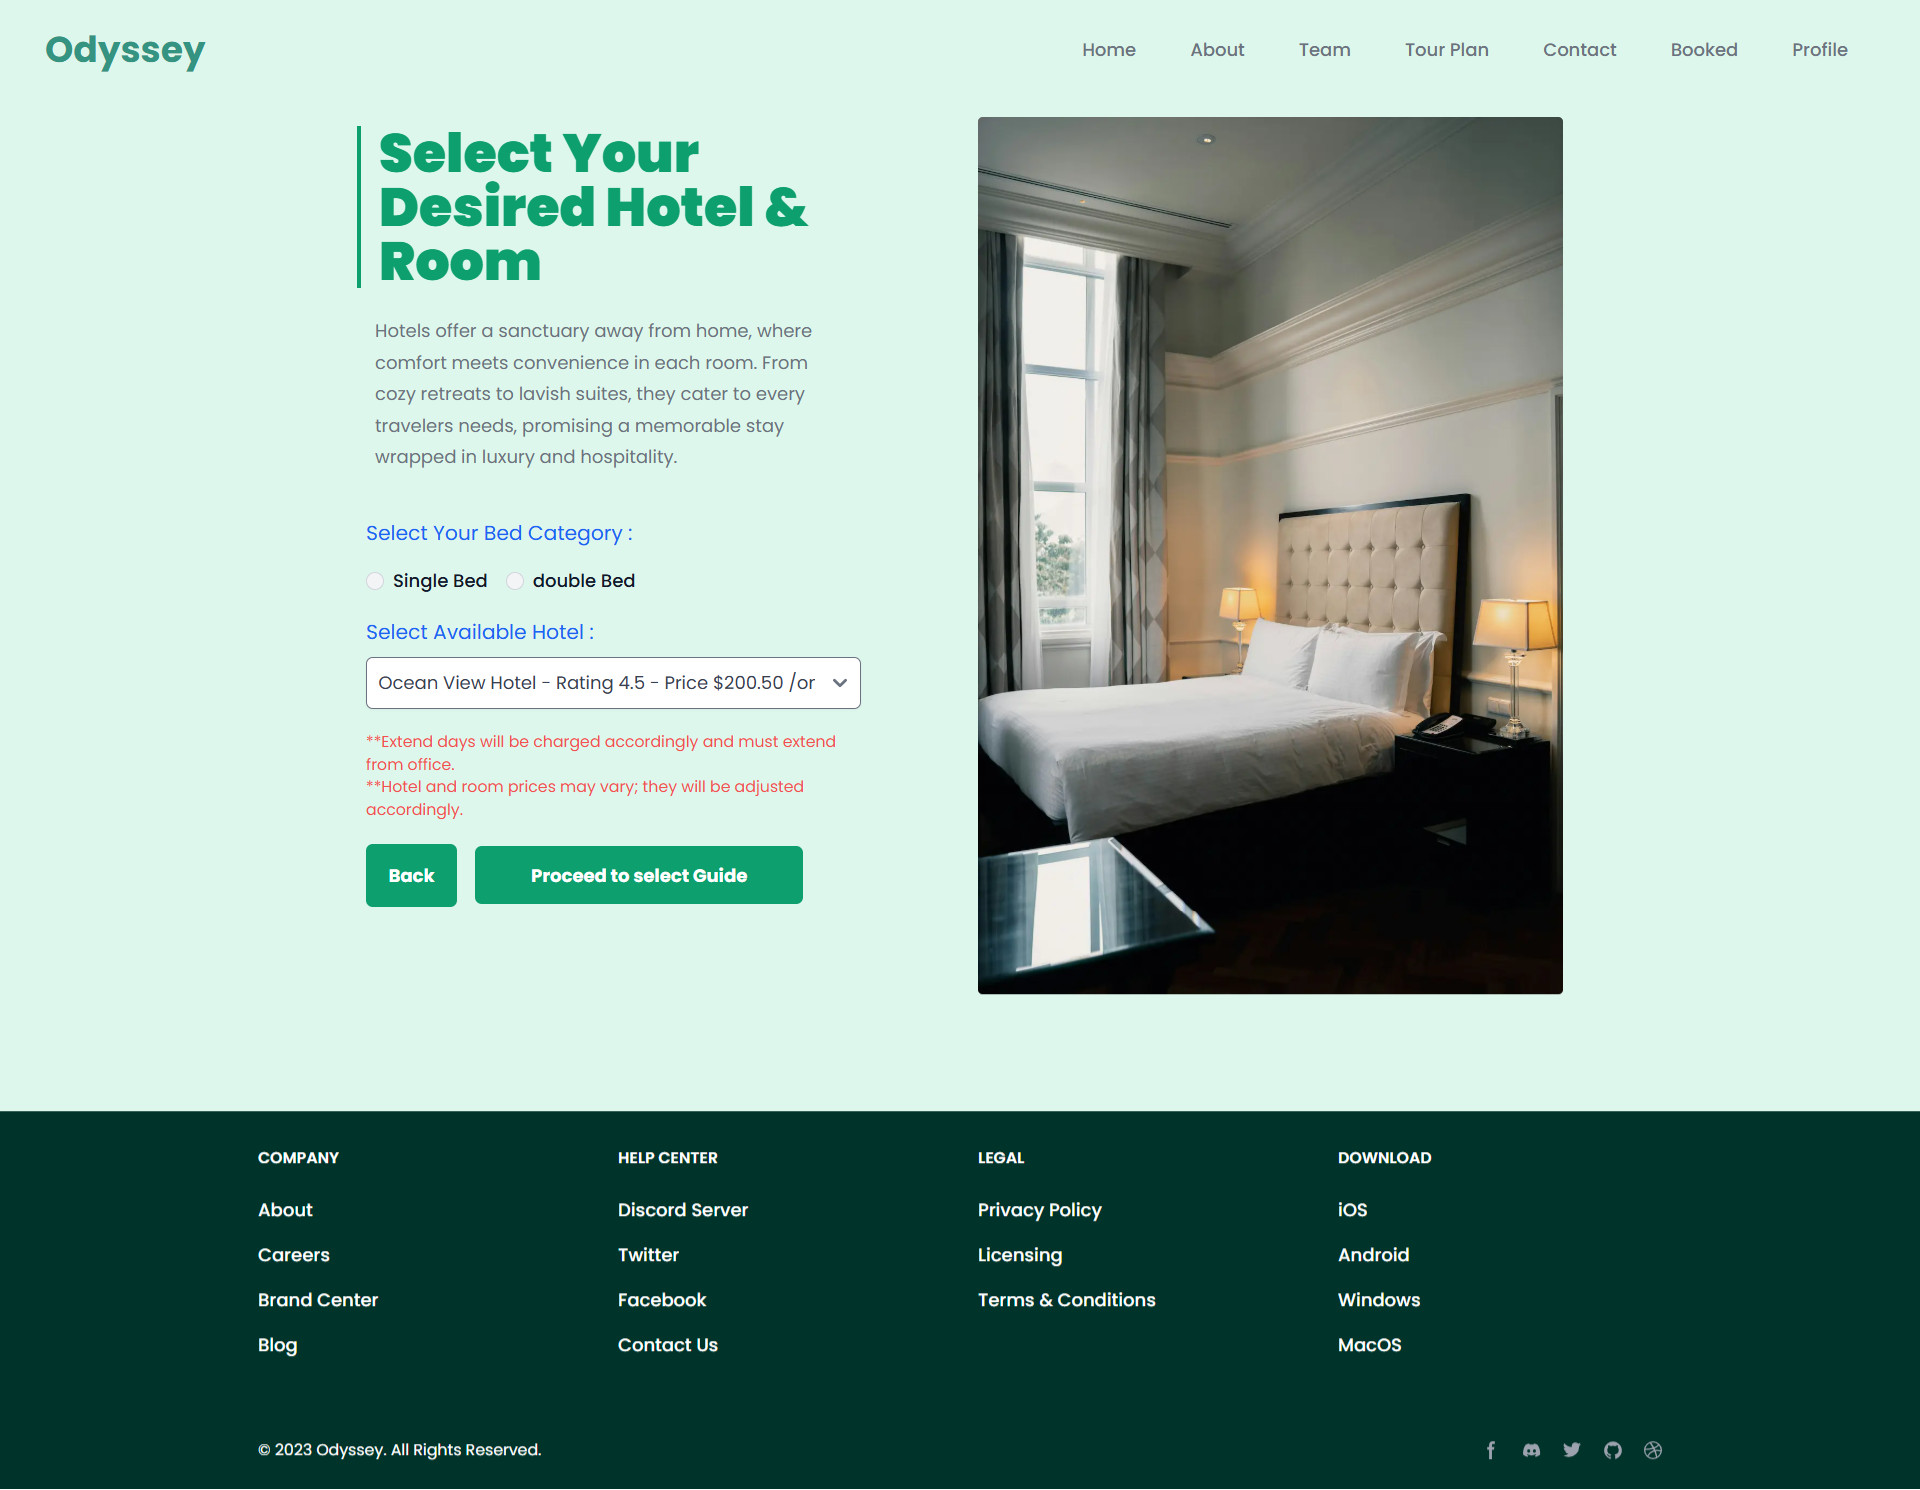
\includegraphics[width=0.95\textwidth]{./figures/frontend/6.png}
    \caption{Select Hotel Page}
    \label{fig:select_hotel}
\end{figure}

\begin{figure}[H]
    \centering
    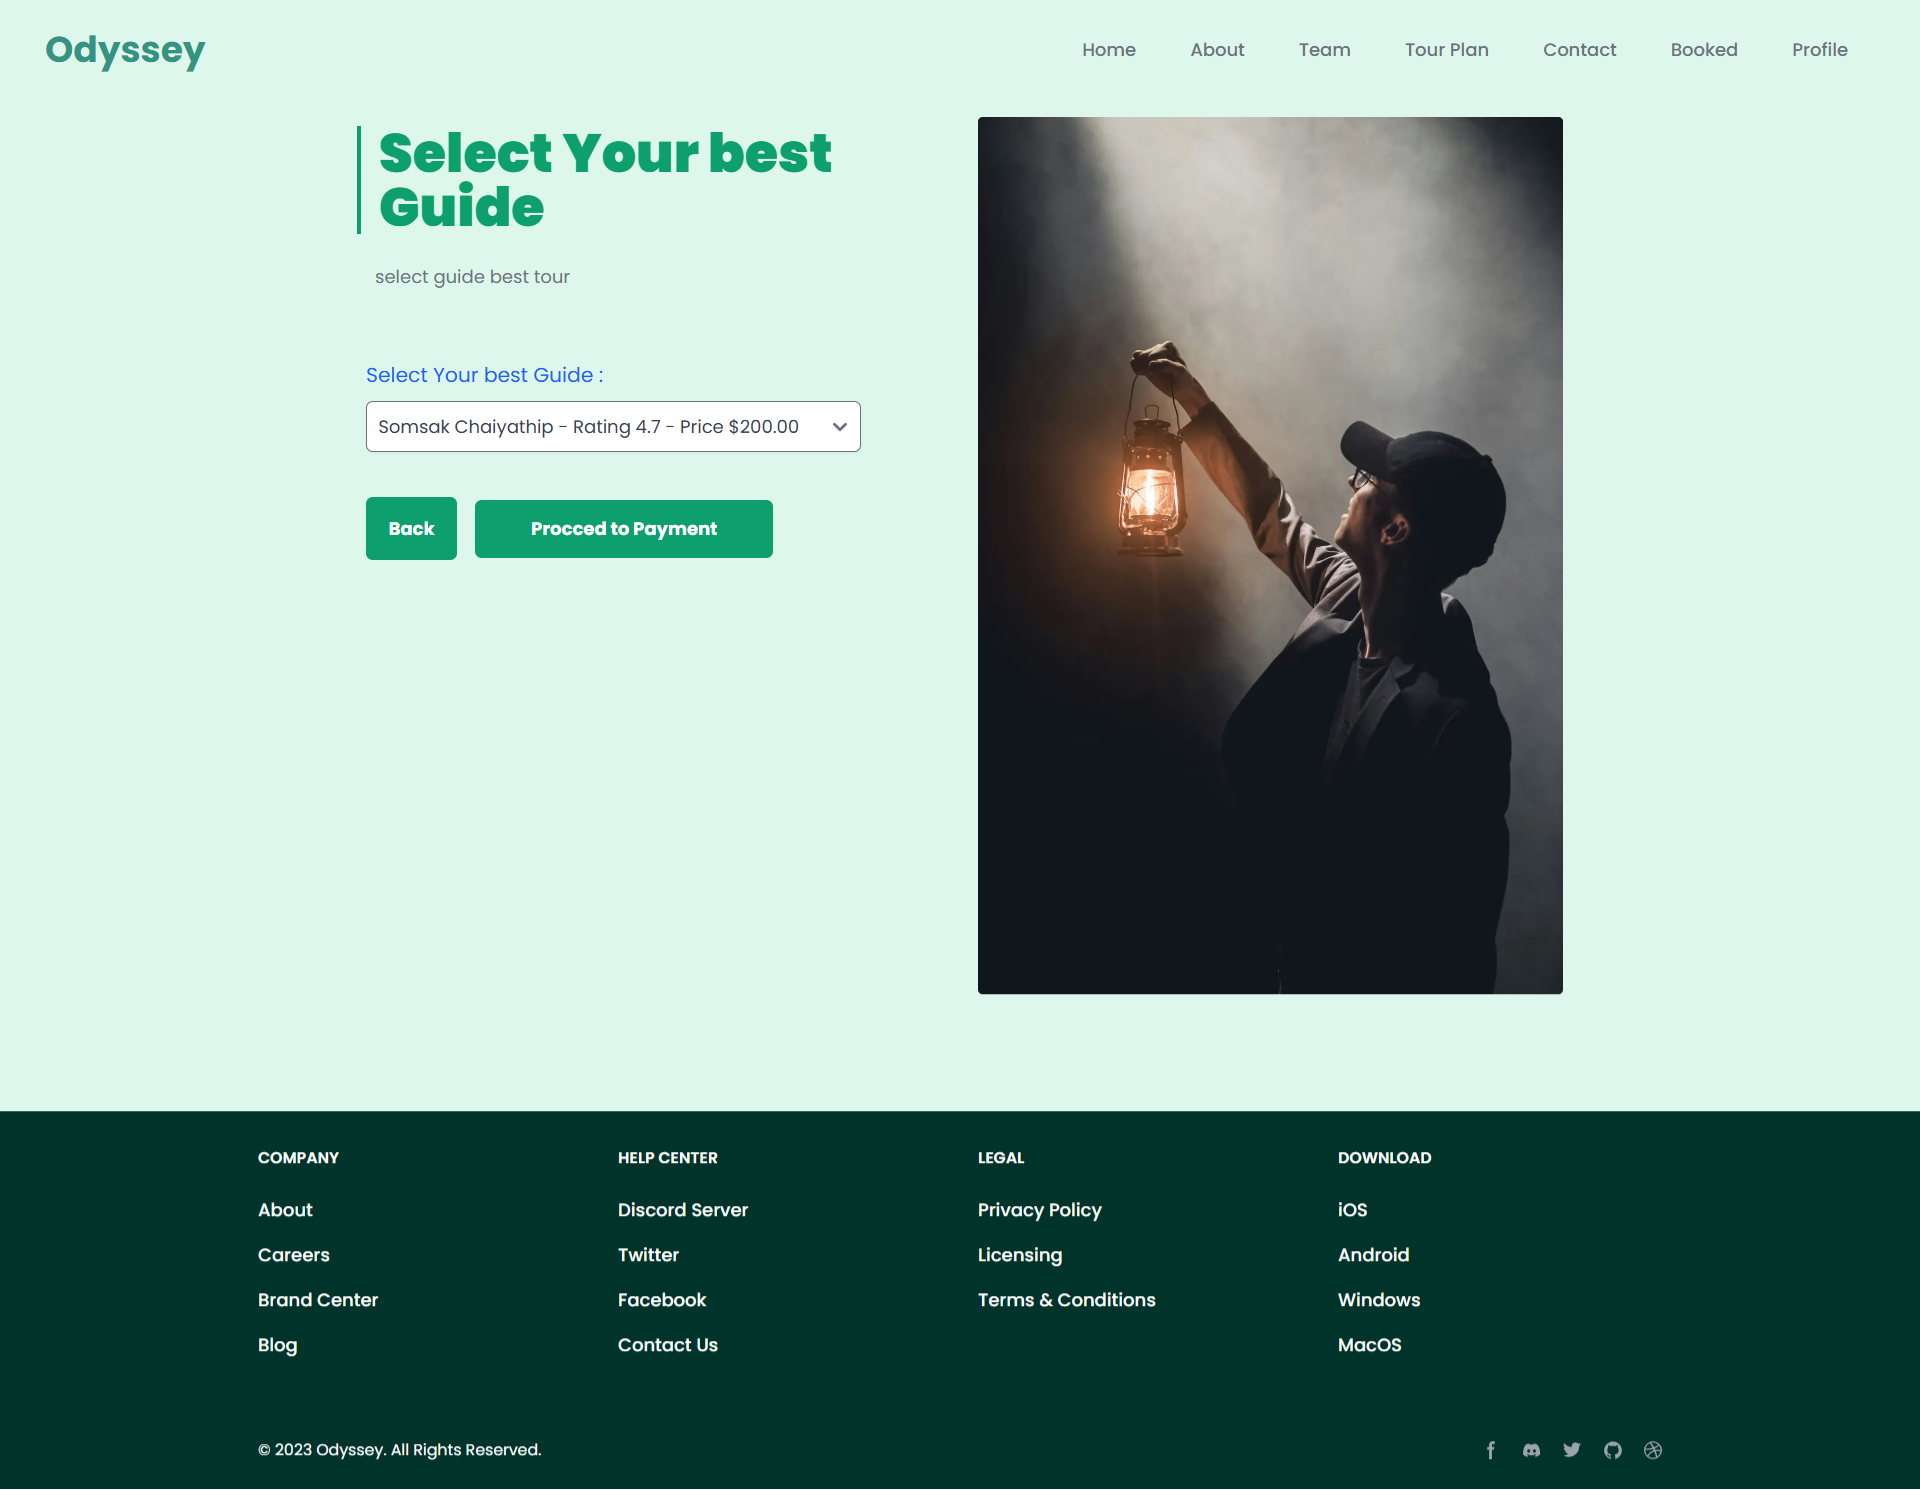
\includegraphics[width=0.95\textwidth]{./figures/frontend/7.png}
    \caption{Select Tour Guide Page}
    \label{fig:select_guide}
\end{figure}

\begin{figure}[H]
    \centering
    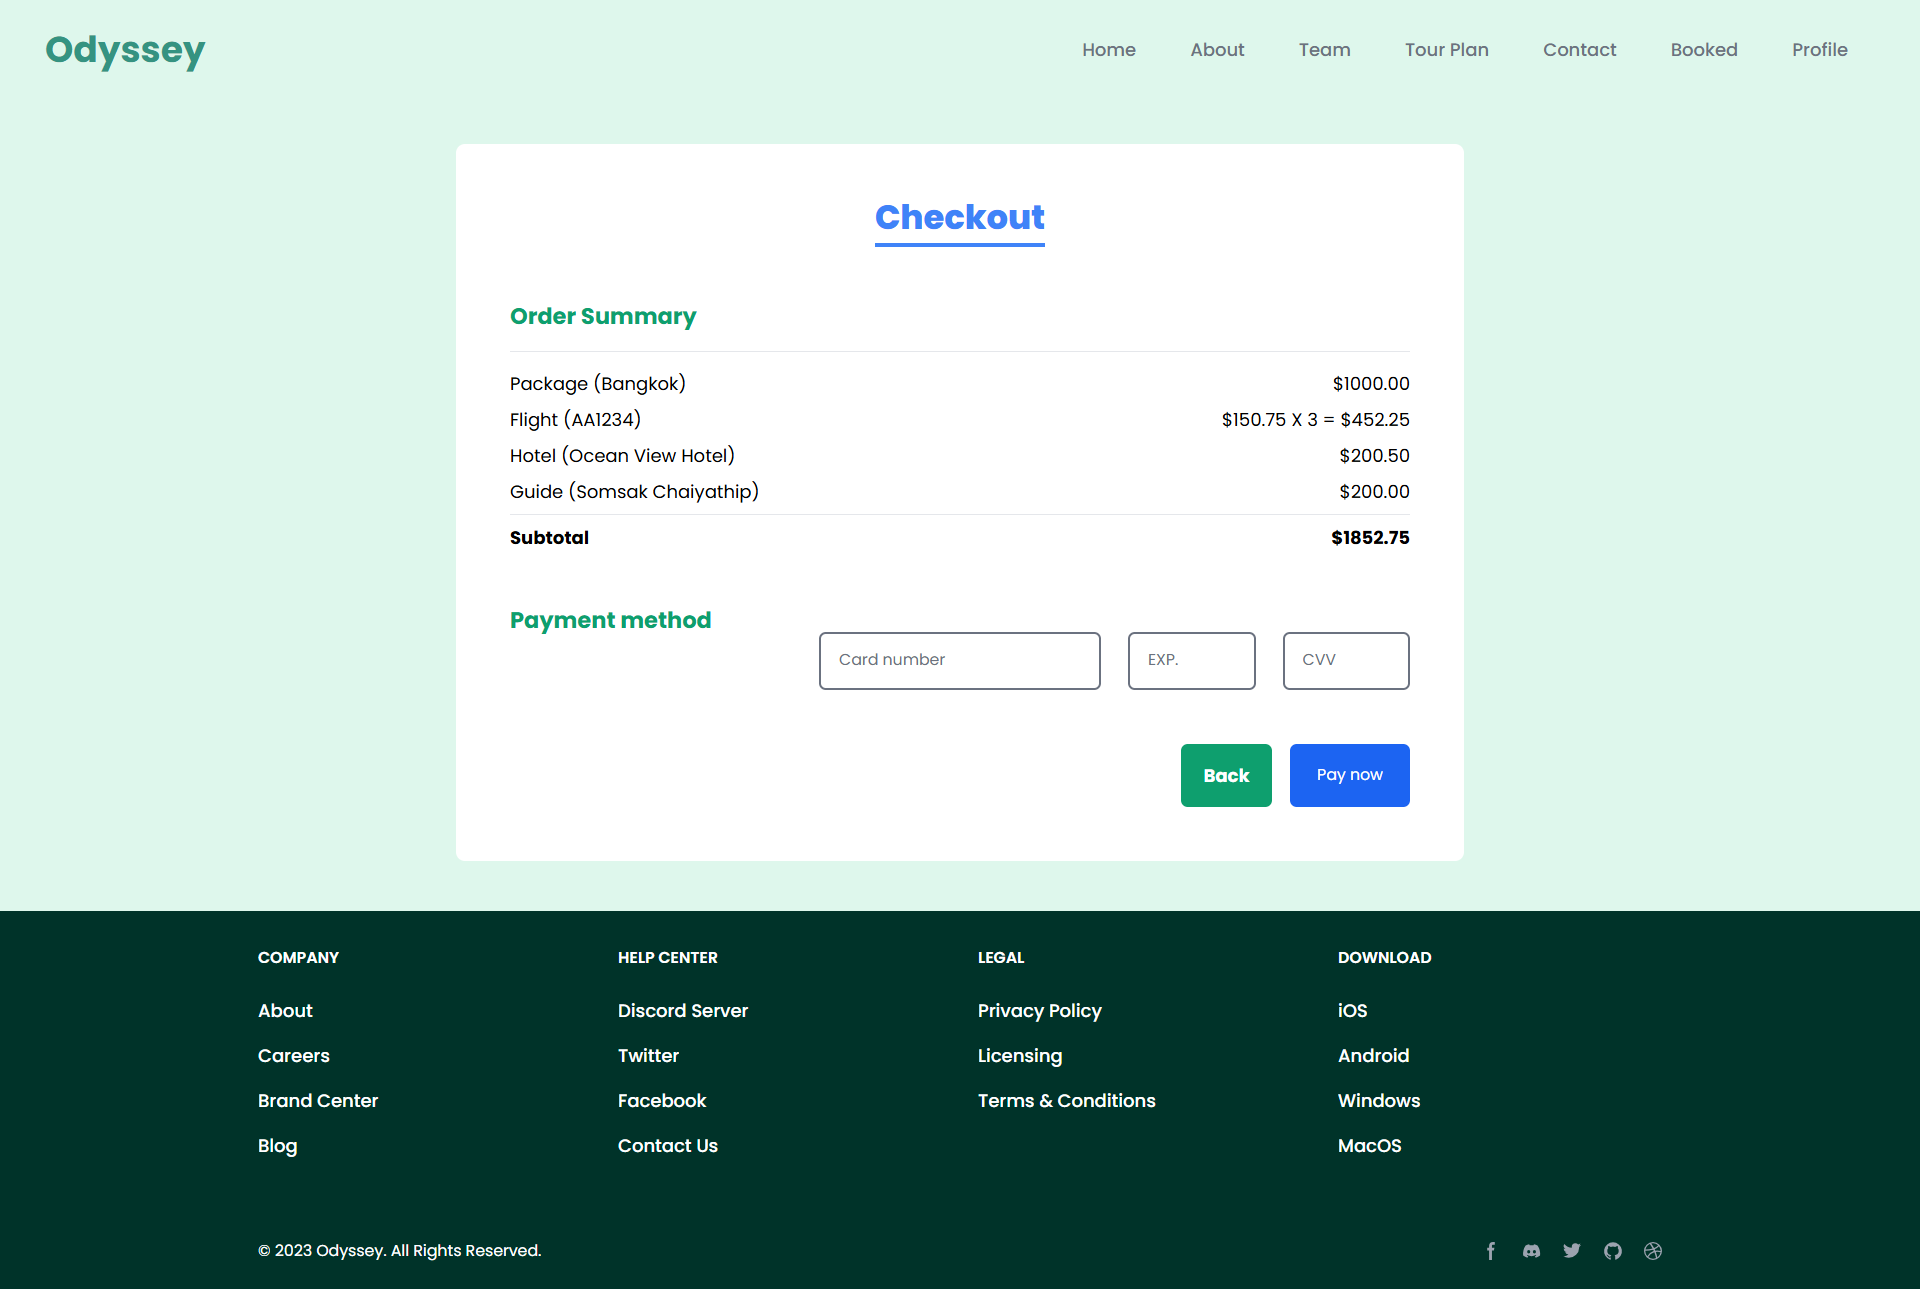
\includegraphics[width=0.95\textwidth]{./figures/frontend/8.png}
    \caption{Payment Checkout Page}
    \label{fig:payment_checkout}
\end{figure}

\begin{figure}[H]
    \centering
    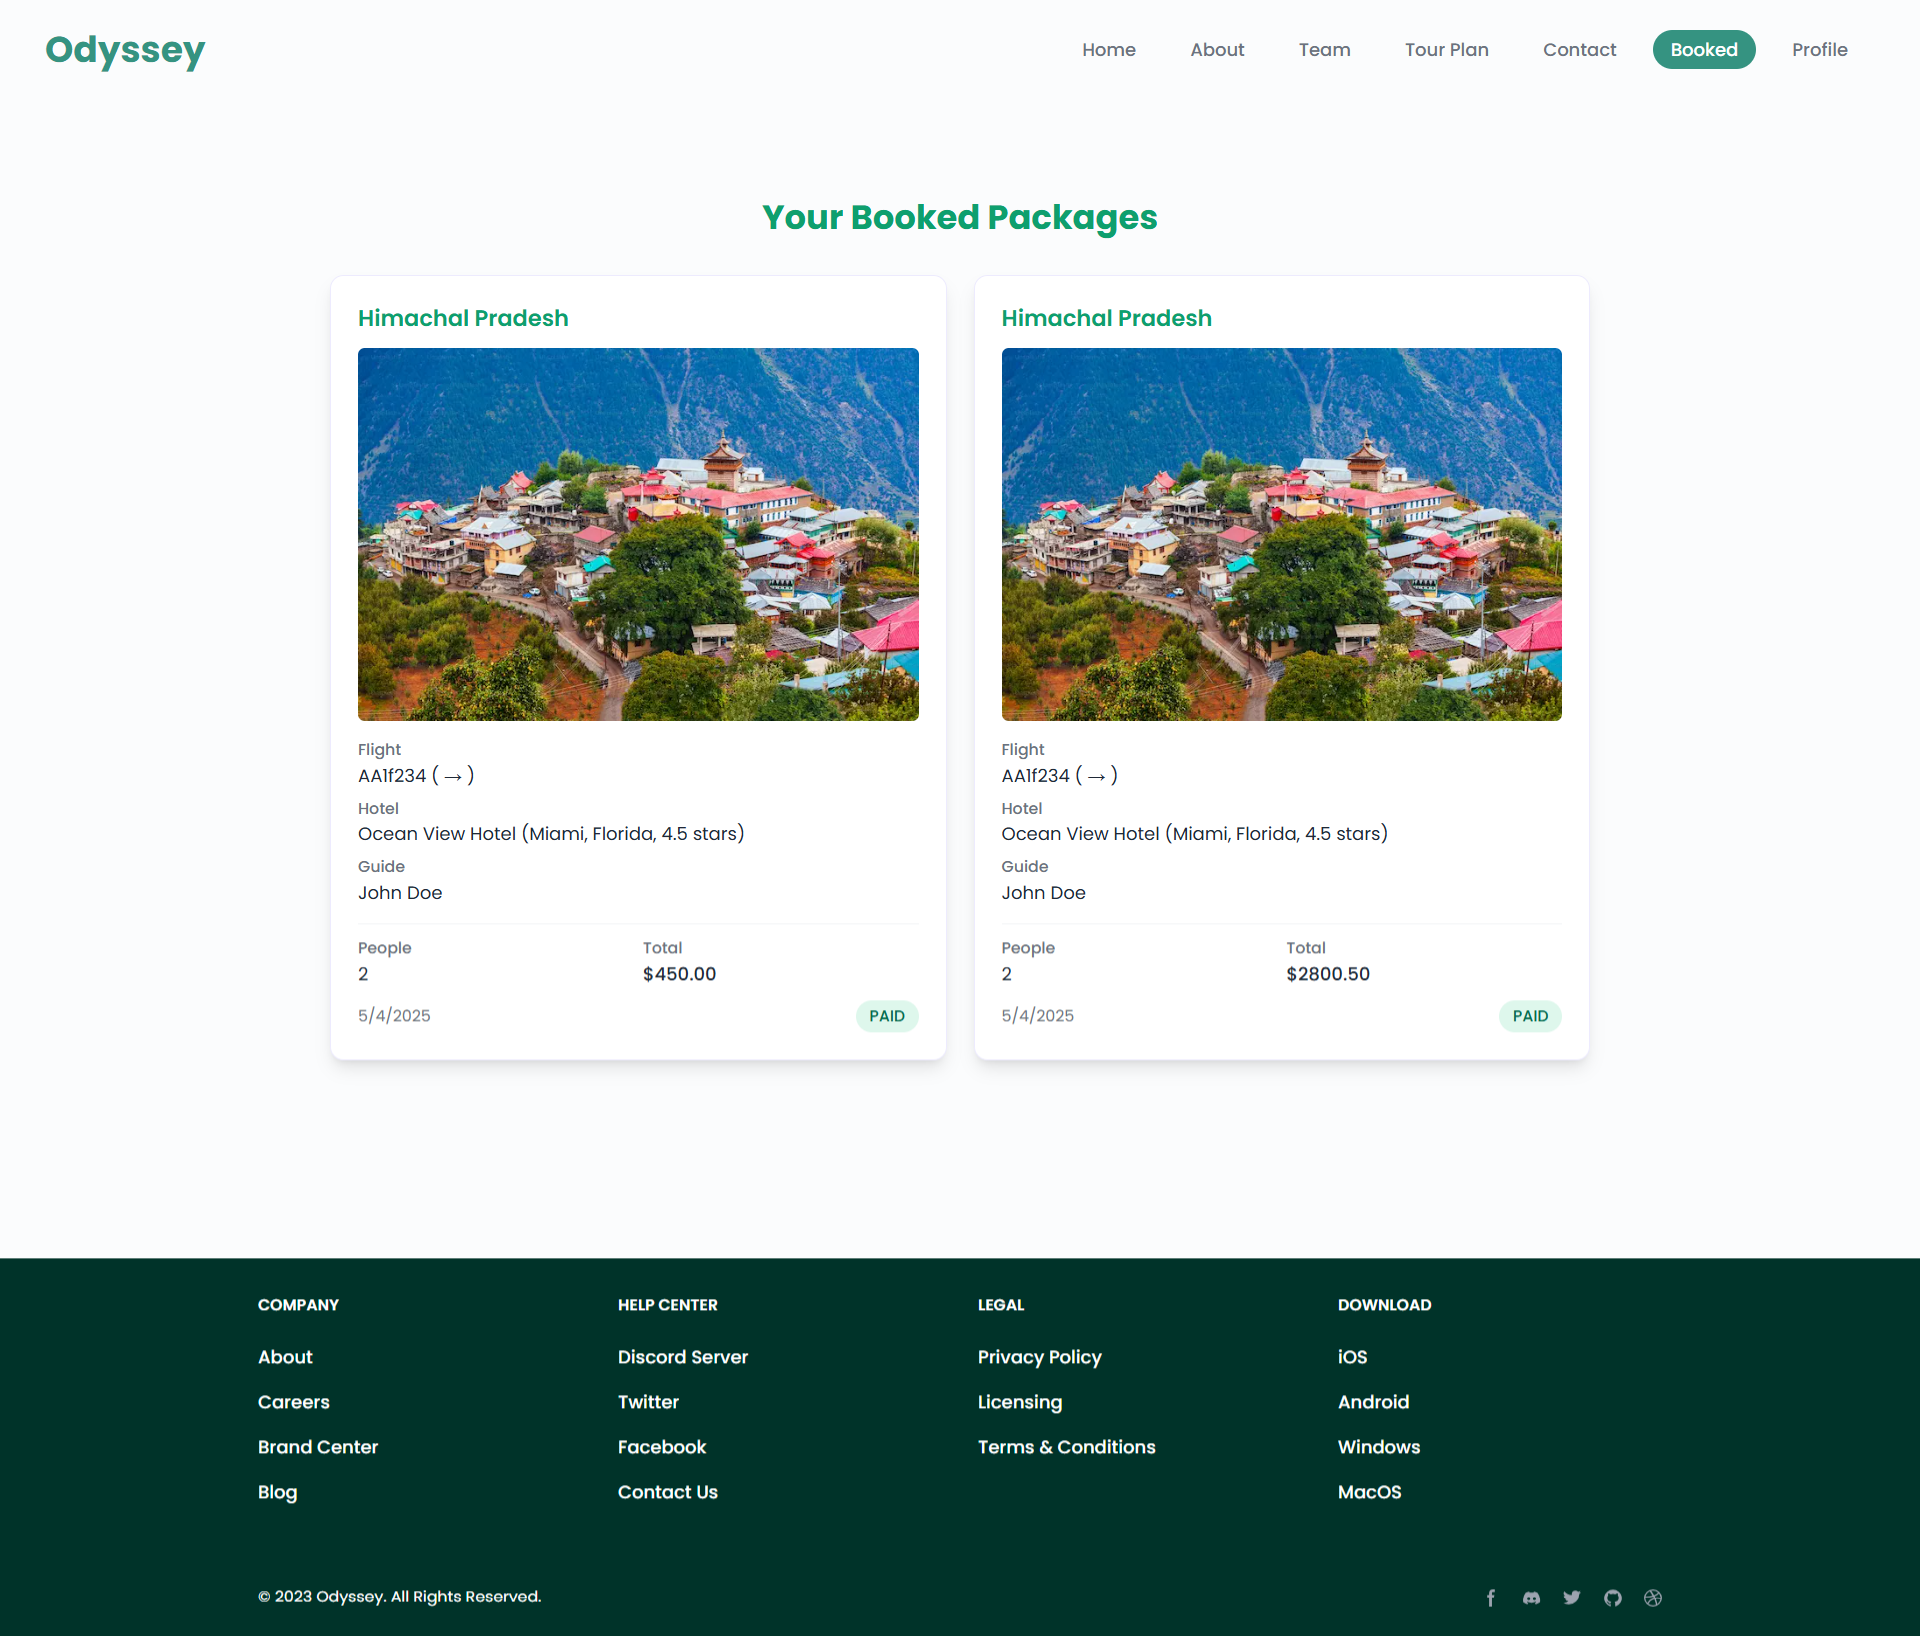
\includegraphics[width=0.95\textwidth]{./figures/frontend/9.png}
    \caption{Order Booking Confirmation Page}
    \label{fig:order_booking}
\end{figure}

\subsection*{Admin Panel Screens}

\begin{figure}[H]
    \centering
    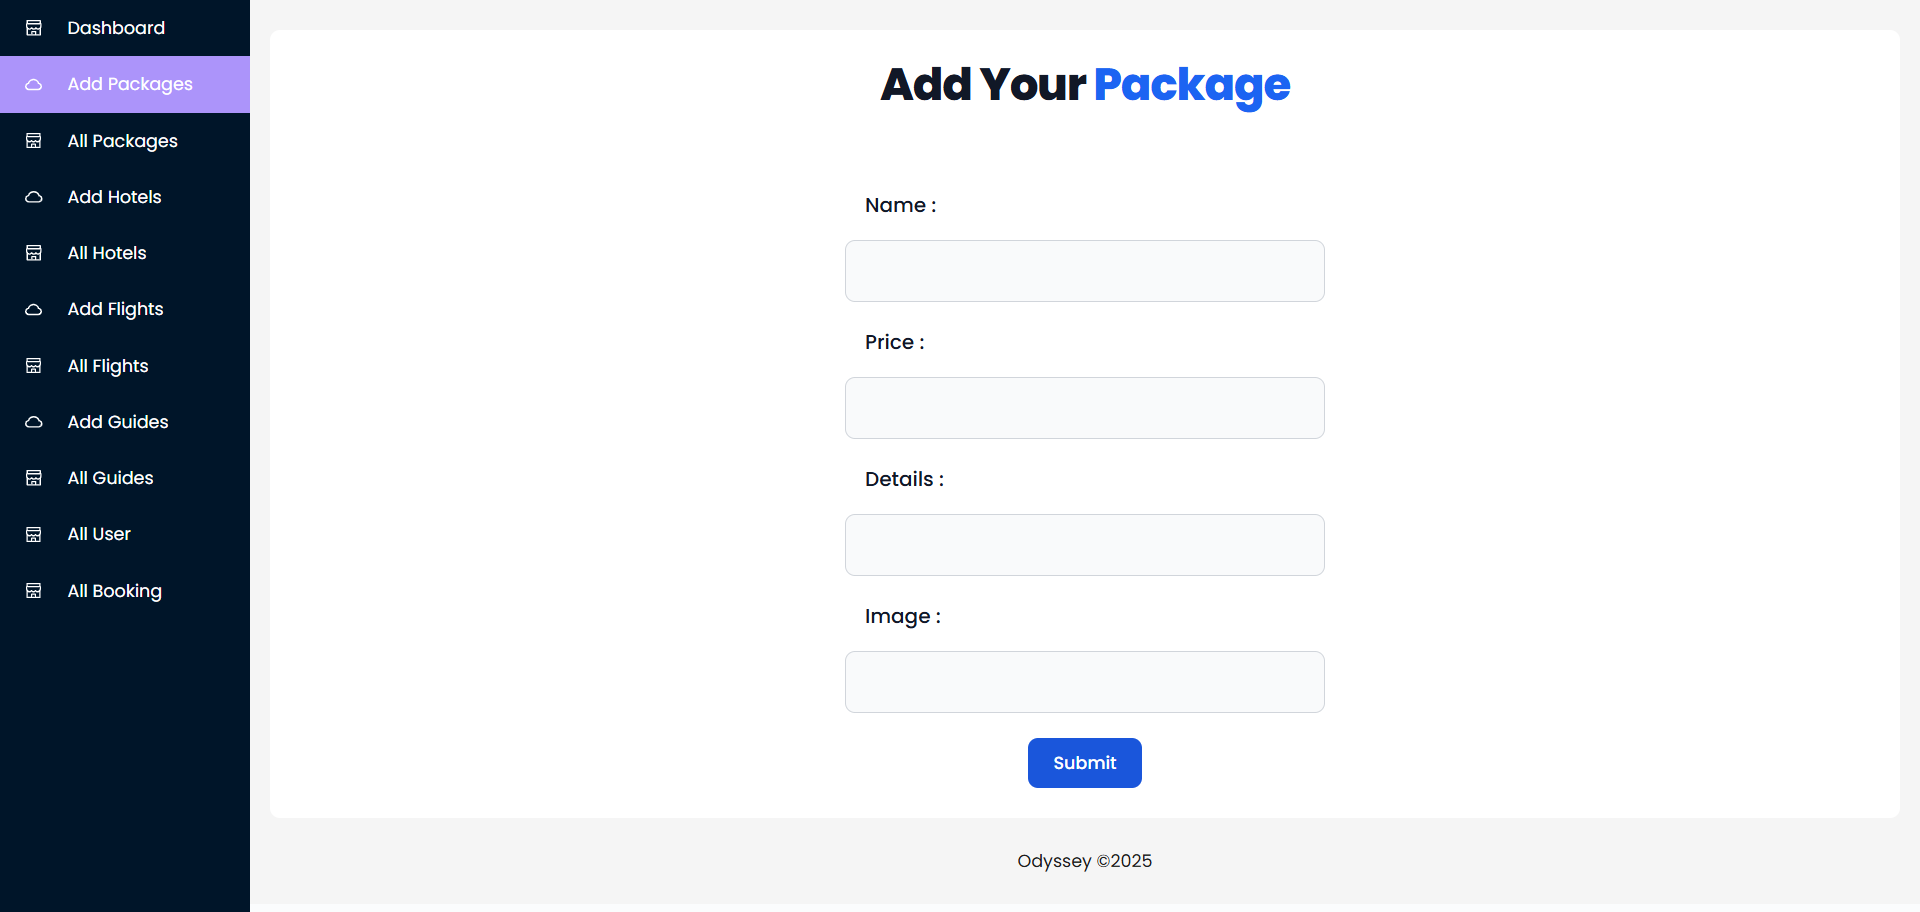
\includegraphics[width=0.95\textwidth]{./figures/frontend/10.png}
    \caption{Add Package (Admin)}
    \label{fig:add_package_admin}
\end{figure}

\begin{figure}[H]
    \centering
    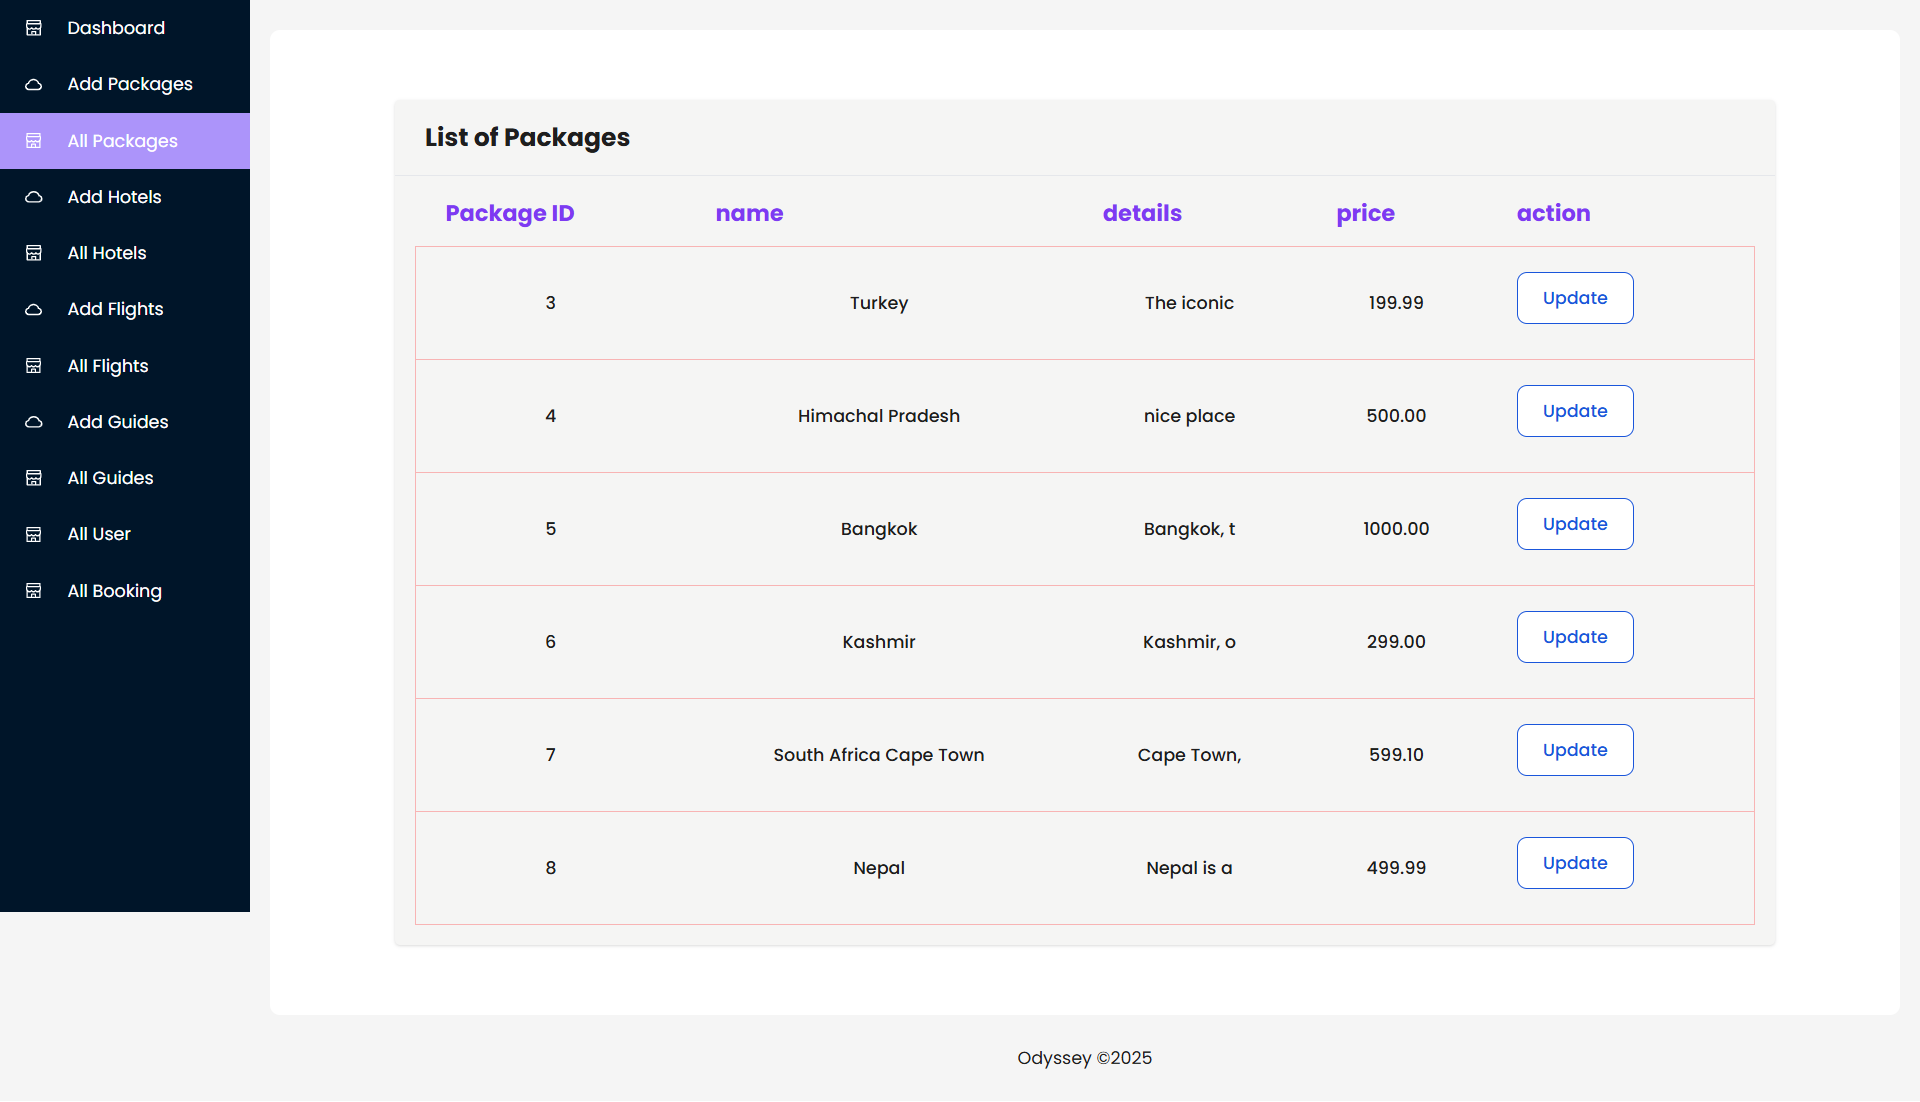
\includegraphics[width=0.95\textwidth]{./figures/frontend/11.png}
    \caption{List of Packages (Admin)}
    \label{fig:list_package_admin}
\end{figure}

\begin{figure}[H]
    \centering
    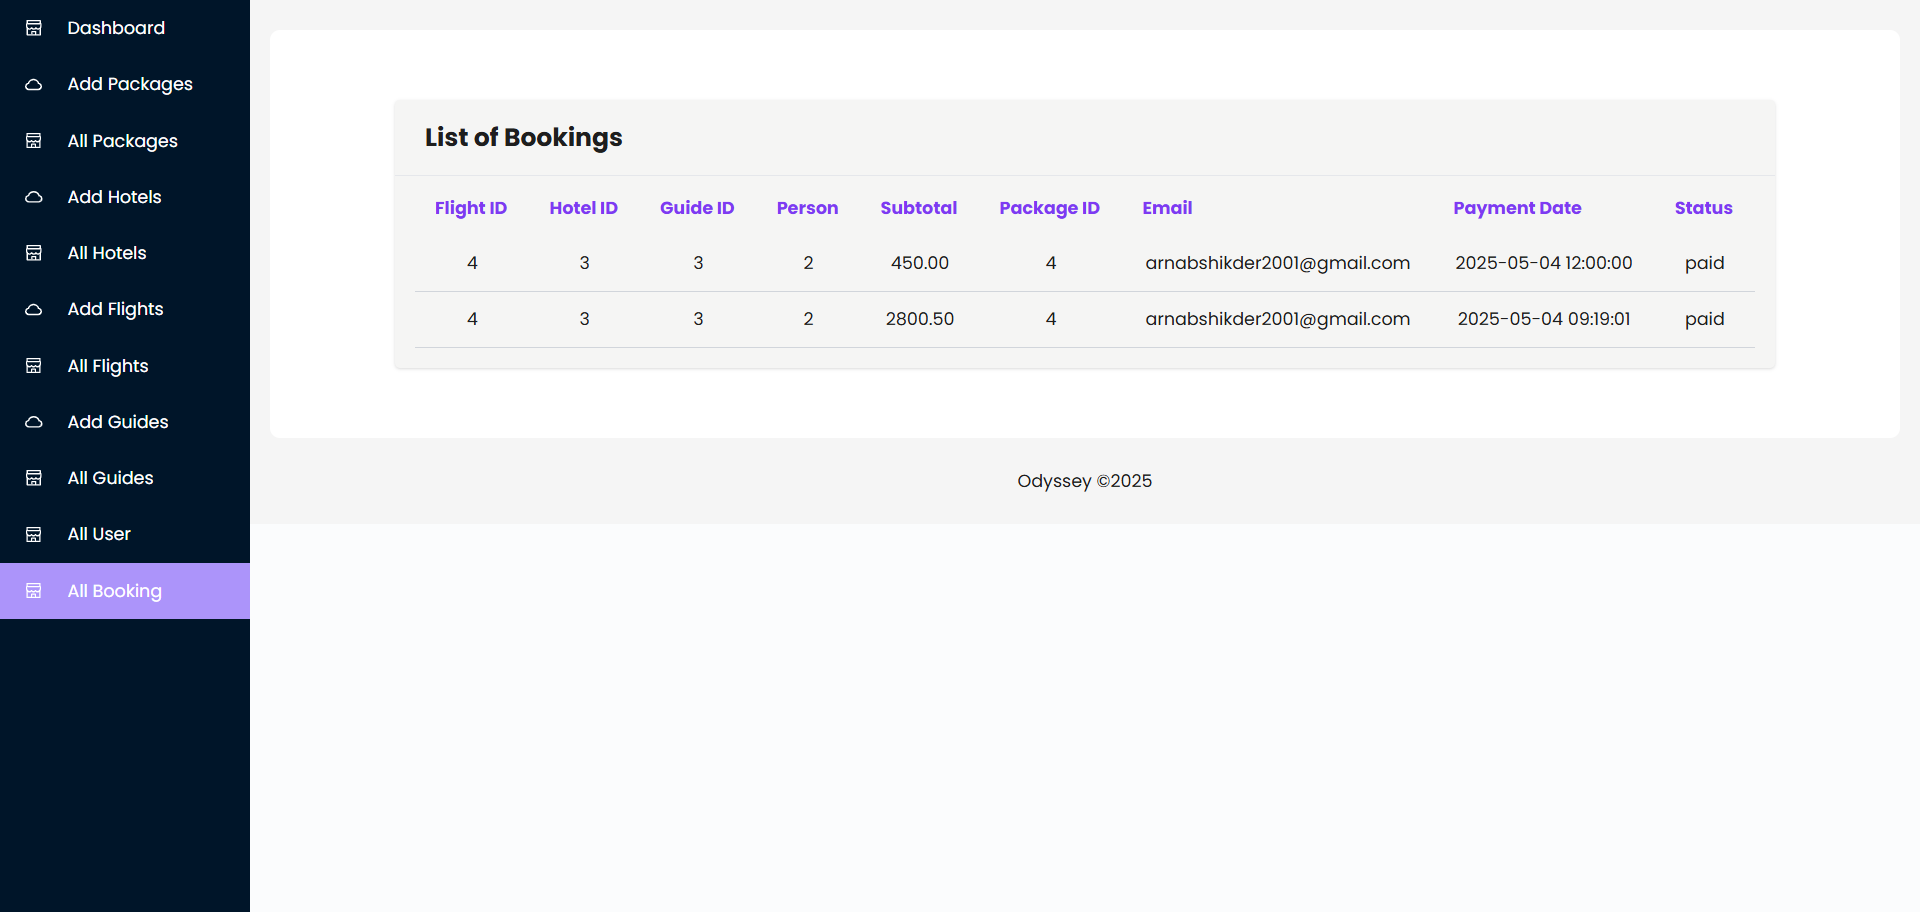
\includegraphics[width=0.95\textwidth]{./figures/frontend/12.png}
    \caption{List of Bookings (Admin)}
    \label{fig:list_bookings_admin}
\end{figure}
